\documentclass[a4paper,12pt]{report}
\usepackage[T1]{fontenc}
\usepackage[polish]{babel}
\usepackage[utf8]{inputenc}
\usepackage{amsmath}
\usepackage{graphicx}

\title{Notatki z wykładu ,,Nieskończone Alfabety''}
% jeśli rozwijasz ten dokument, dopisz się do listy autorów
% porządek autorów powinien być alfabetyczny
\author{Tomasz Wysocki}
\begin{document}
\maketitle
\newpage
\tableofcontents
\newpage
\chapter {Wykład I: wstęp do nieskończonych alfabetów}
\section {Dlaczego warto badać nieskończone alfabety?}
\section {Znane modele automatów dla słów}
\begin{figure}
\begin{center}
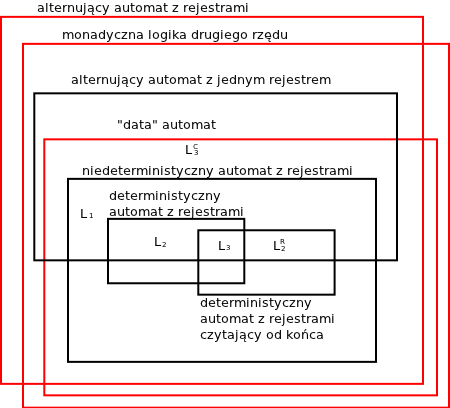
\includegraphics{images/podzial_automatow.png}
\end{center}
\caption{Moc wyrazu poszczególnych modeli}
\end{figure}

\section {Definicja niedeterministycznego automatu z rejestrami}
\end{document}